% GNUPLOT: LaTeX picture with Postscript
\begingroup
  \makeatletter
  \providecommand\color[2][]{%
    \GenericError{(gnuplot) \space\space\space\@spaces}{%
      Package color not loaded in conjunction with
      terminal option `colourtext'%
    }{See the gnuplot documentation for explanation.%
    }{Either use 'blacktext' in gnuplot or load the package
      color.sty in LaTeX.}%
    \renewcommand\color[2][]{}%
  }%
  \providecommand\includegraphics[2][]{%
    \GenericError{(gnuplot) \space\space\space\@spaces}{%
      Package graphicx or graphics not loaded%
    }{See the gnuplot documentation for explanation.%
    }{The gnuplot epslatex terminal needs graphicx.sty or graphics.sty.}%
    \renewcommand\includegraphics[2][]{}%
  }%
  \providecommand\rotatebox[2]{#2}%
  \@ifundefined{ifGPcolor}{%
    \newif\ifGPcolor
    \GPcolortrue
  }{}%
  \@ifundefined{ifGPblacktext}{%
    \newif\ifGPblacktext
    \GPblacktexttrue
  }{}%
  % define a \g@addto@macro without @ in the name:
  \let\gplgaddtomacro\g@addto@macro
  % define empty templates for all commands taking text:
  \gdef\gplbacktext{}%
  \gdef\gplfronttext{}%
  \makeatother
  \ifGPblacktext
    % no textcolor at all
    \def\colorrgb#1{}%
    \def\colorgray#1{}%
  \else
    % gray or color?
    \ifGPcolor
      \def\colorrgb#1{\color[rgb]{#1}}%
      \def\colorgray#1{\color[gray]{#1}}%
      \expandafter\def\csname LTw\endcsname{\color{white}}%
      \expandafter\def\csname LTb\endcsname{\color{black}}%
      \expandafter\def\csname LTa\endcsname{\color{black}}%
      \expandafter\def\csname LT0\endcsname{\color[rgb]{1,0,0}}%
      \expandafter\def\csname LT1\endcsname{\color[rgb]{0,1,0}}%
      \expandafter\def\csname LT2\endcsname{\color[rgb]{0,0,1}}%
      \expandafter\def\csname LT3\endcsname{\color[rgb]{1,0,1}}%
      \expandafter\def\csname LT4\endcsname{\color[rgb]{0,1,1}}%
      \expandafter\def\csname LT5\endcsname{\color[rgb]{1,1,0}}%
      \expandafter\def\csname LT6\endcsname{\color[rgb]{0,0,0}}%
      \expandafter\def\csname LT7\endcsname{\color[rgb]{1,0.3,0}}%
      \expandafter\def\csname LT8\endcsname{\color[rgb]{0.5,0.5,0.5}}%
    \else
      % gray
      \def\colorrgb#1{\color{black}}%
      \def\colorgray#1{\color[gray]{#1}}%
      \expandafter\def\csname LTw\endcsname{\color{white}}%
      \expandafter\def\csname LTb\endcsname{\color{black}}%
      \expandafter\def\csname LTa\endcsname{\color{black}}%
      \expandafter\def\csname LT0\endcsname{\color{black}}%
      \expandafter\def\csname LT1\endcsname{\color{black}}%
      \expandafter\def\csname LT2\endcsname{\color{black}}%
      \expandafter\def\csname LT3\endcsname{\color{black}}%
      \expandafter\def\csname LT4\endcsname{\color{black}}%
      \expandafter\def\csname LT5\endcsname{\color{black}}%
      \expandafter\def\csname LT6\endcsname{\color{black}}%
      \expandafter\def\csname LT7\endcsname{\color{black}}%
      \expandafter\def\csname LT8\endcsname{\color{black}}%
    \fi
  \fi
    \setlength{\unitlength}{0.0500bp}%
    \ifx\gptboxheight\undefined%
      \newlength{\gptboxheight}%
      \newlength{\gptboxwidth}%
      \newsavebox{\gptboxtext}%
    \fi%
    \setlength{\fboxrule}{0.5pt}%
    \setlength{\fboxsep}{1pt}%
\begin{picture}(14400.00,5040.00)%
    \gplgaddtomacro\gplbacktext{%
      \csname LTb\endcsname%%
      \put(444,972){\makebox(0,0)[r]{\strut{}\np{e-1}}}%
      \put(444,2740){\makebox(0,0)[r]{\strut{}\np{e0}}}%
      \put(444,4507){\makebox(0,0)[r]{\strut{}\np{e1}}}%
      \put(576,220){\makebox(0,0){\strut{}\np{e-10}}}%
      \put(1497,220){\makebox(0,0){\strut{}\np{e-8}}}%
      \put(2419,220){\makebox(0,0){\strut{}\np{e-6}}}%
      \put(3340,220){\makebox(0,0){\strut{}\np{e-4}}}%
      \put(4262,220){\makebox(0,0){\strut{}\np{e-2}}}%
    }%
    \gplgaddtomacro\gplfronttext{%
      \csname LTb\endcsname%%
      \put(-304,2739){\rotatebox{-270}{\makebox(0,0){\strut{}$\Delta m_{4 1}^2 $}}}%
      \put(2879,-110){\makebox(0,0){\strut{}$|U_{e 4}|^2$}}%
      \csname LTb\endcsname%%
      \put(1167,4844){\makebox(0,0)[l]{\strut{}DANSS}}%
      \csname LTb\endcsname%%
      \put(1167,4580){\makebox(0,0)[l]{\strut{}NEOS}}%
      \csname LTb\endcsname%%
      \put(1167,4316){\makebox(0,0)[l]{\strut{}STEREO}}%
      \csname LTb\endcsname%%
      \put(1167,4052){\makebox(0,0)[l]{\strut{}SK + IC}}%
    }%
    \gplgaddtomacro\gplbacktext{%
      \csname LTb\endcsname%%
      \put(5052,972){\makebox(0,0)[r]{\strut{}}}%
      \put(5052,2740){\makebox(0,0)[r]{\strut{}}}%
      \put(5052,4507){\makebox(0,0)[r]{\strut{}}}%
      \put(5184,220){\makebox(0,0){\strut{}\np{e-12}}}%
      \put(5952,220){\makebox(0,0){\strut{}\np{e-10}}}%
      \put(6720,220){\makebox(0,0){\strut{}\np{e-8}}}%
      \put(7488,220){\makebox(0,0){\strut{}\np{e-6}}}%
      \put(8255,220){\makebox(0,0){\strut{}\np{e-4}}}%
      \put(9023,220){\makebox(0,0){\strut{}\np{e-2}}}%
    }%
    \gplgaddtomacro\gplfronttext{%
      \csname LTb\endcsname%%
      \put(7487,-110){\makebox(0,0){\strut{}$4 |U_{e 4}|^2 |U_{\mu 4}|^2$}}%
      \csname LTb\endcsname%%
      \put(5775,4844){\makebox(0,0)[l]{\strut{}MiniBooNE}}%
      \csname LTb\endcsname%%
      \put(5775,4580){\makebox(0,0)[l]{\strut{}KARMEN}}%
      \csname LTb\endcsname%%
      \put(5775,4316){\makebox(0,0)[l]{\strut{}OPERA}}%
    }%
    \gplgaddtomacro\gplbacktext{%
      \csname LTb\endcsname%%
      \put(9660,972){\makebox(0,0)[r]{\strut{}}}%
      \put(9660,2740){\makebox(0,0)[r]{\strut{}}}%
      \put(9660,4507){\makebox(0,0)[r]{\strut{}}}%
      \put(14399,220){\makebox(0,0){\strut{}\np{e0}}}%
      \put(9792,220){\makebox(0,0){\strut{}\np{e-10}}}%
      \put(10713,220){\makebox(0,0){\strut{}\np{e-8}}}%
      \put(11635,220){\makebox(0,0){\strut{}\np{e-6}}}%
      \put(12556,220){\makebox(0,0){\strut{}\np{e-4}}}%
      \put(13478,220){\makebox(0,0){\strut{}\np{e-2}}}%
    }%
    \gplgaddtomacro\gplfronttext{%
      \csname LTb\endcsname%%
      \put(12095,-110){\makebox(0,0){\strut{}$|U_{\mu 4}|^2$}}%
      \csname LTb\endcsname%%
      \put(10383,4844){\makebox(0,0)[l]{\strut{}$\nu_\mu\to\nu_\mu$}}%
    }%
    \gplbacktext
    \put(0,0){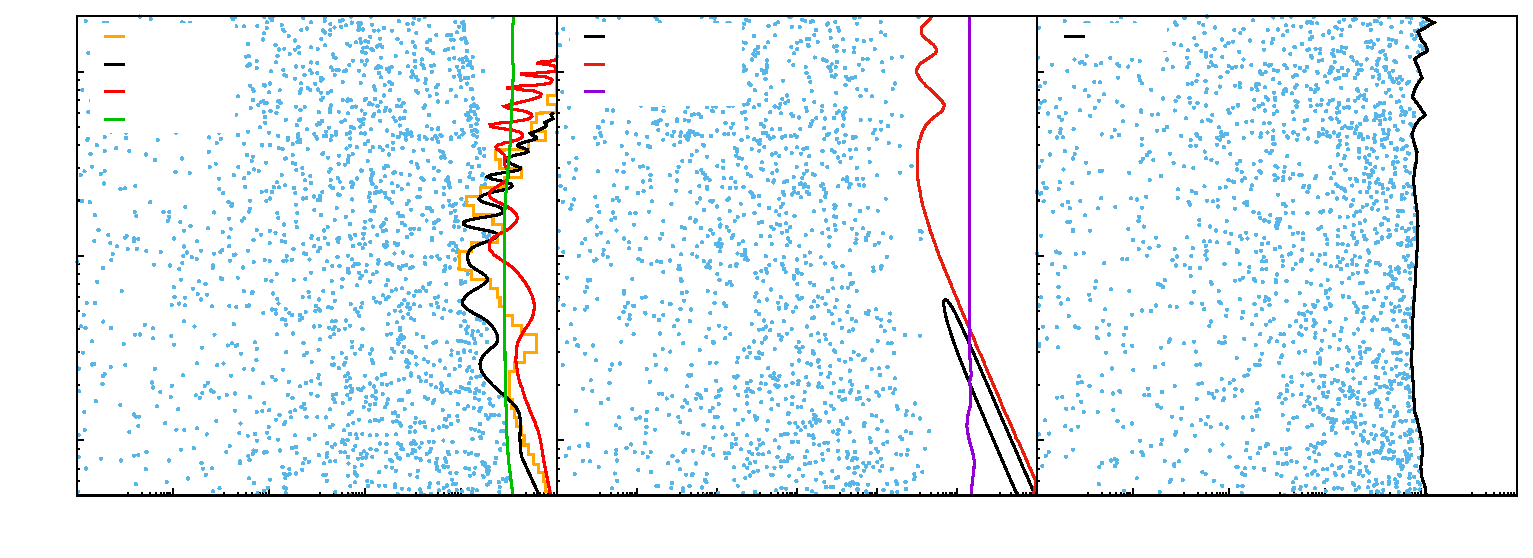
\includegraphics{pics/multiSBL}}%
    \gplfronttext
  \end{picture}%
\endgroup
